\chapter{Function Declaration} % (fold)
\label{cha:function_declaration}

\minitoc

% ============
% = Concepts =
% ============

\section{Function Concepts} % (fold)
\label{sec:function_concepts}

\clearpage
\subsection{Function} % (fold)
\label{sub:function}

\begin{figure}[h]
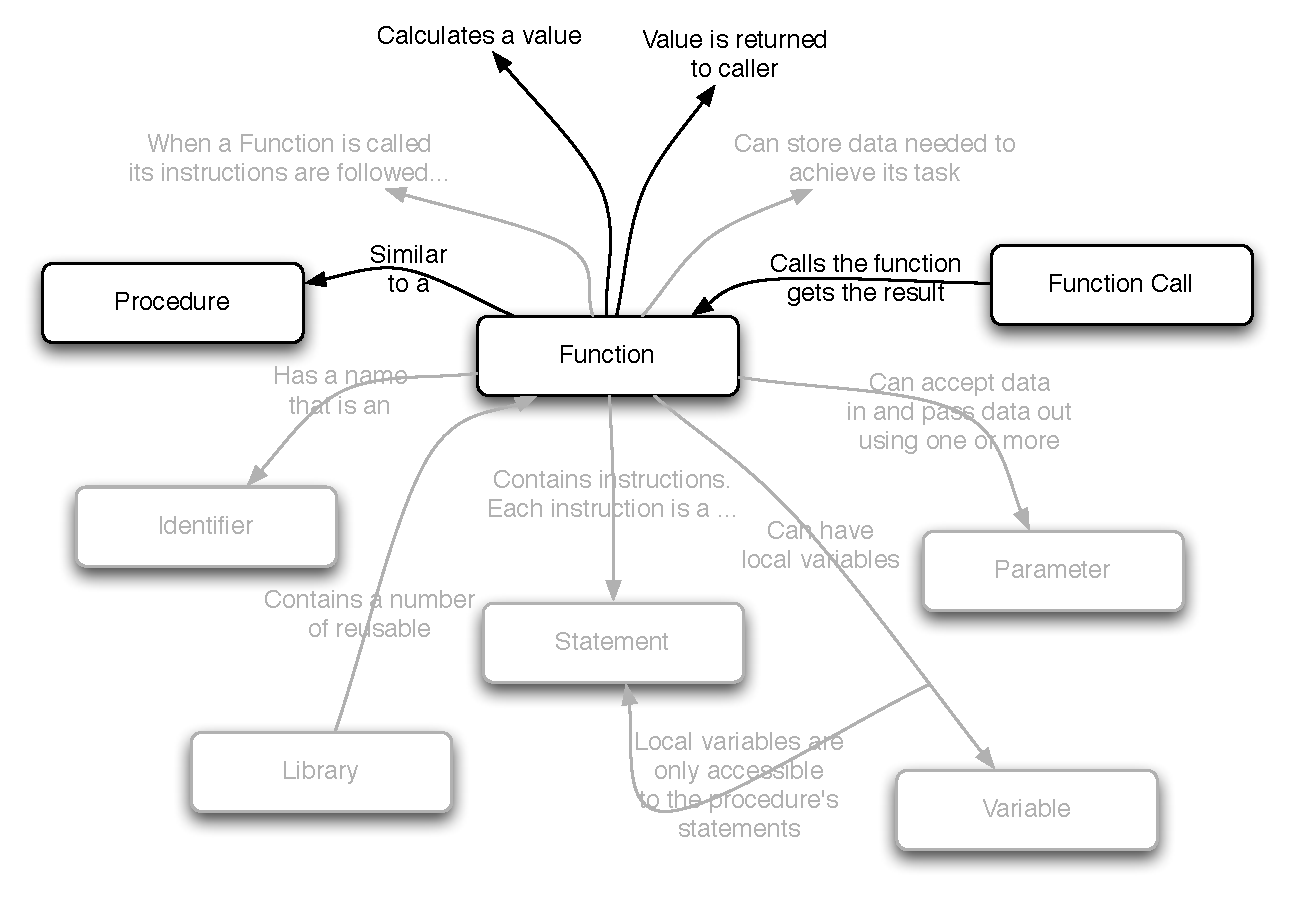
\includegraphics[width=\textwidth]{topics/function-decl/diagrams/Function} 
 \caption{Concepts related to Functions}
 \label{fig:function-decl-function}
\end{figure}


% subsection function (end)
\clearpage
\subsection{Function Call} % (fold)
\label{sub:function_call}

\begin{figure}[h]
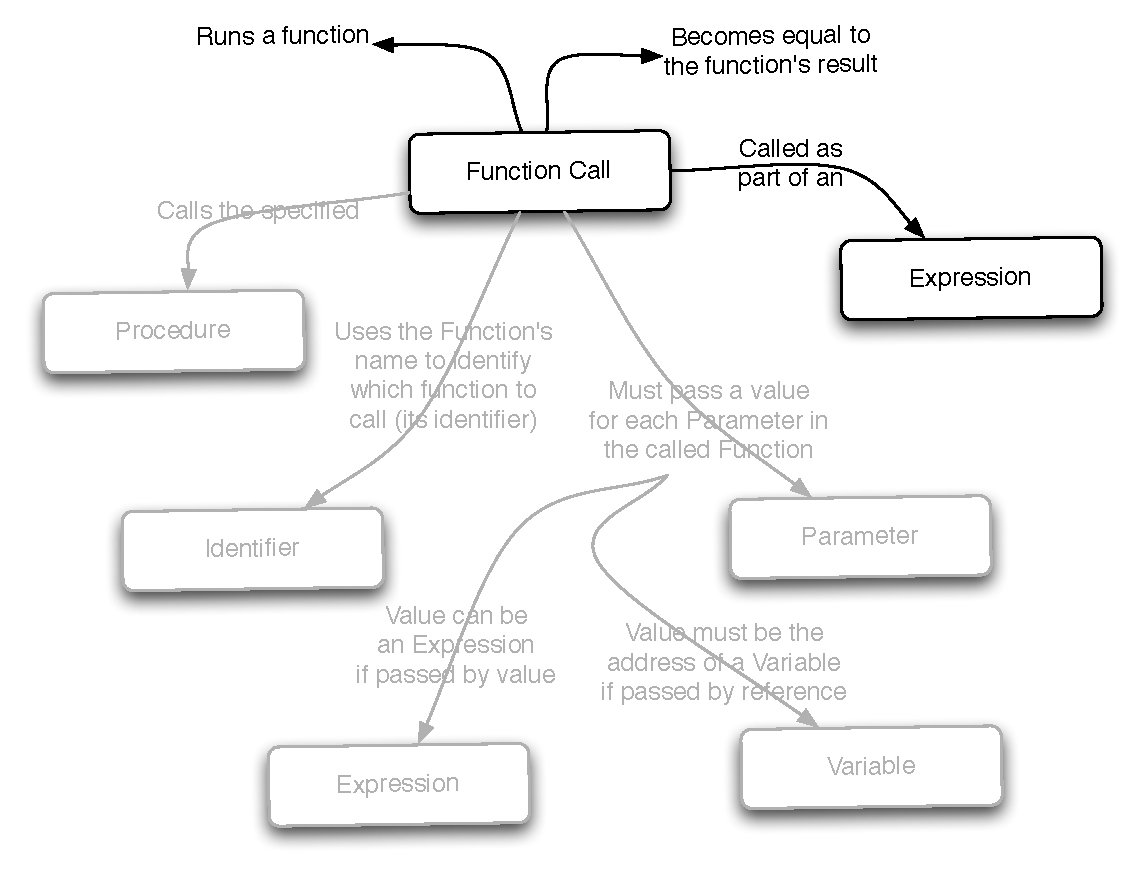
\includegraphics[width=\textwidth]{topics/function-decl/diagrams/FunctionCall} 
 \caption{Concepts related to calling a Function}
 \label{fig:function-decl-function-call}
\end{figure}


% subsection function_call (end)
\clearpage
\subsection{Program (with functions)} % (fold)
\label{sub:program_with_functions_}

\begin{figure}[h]
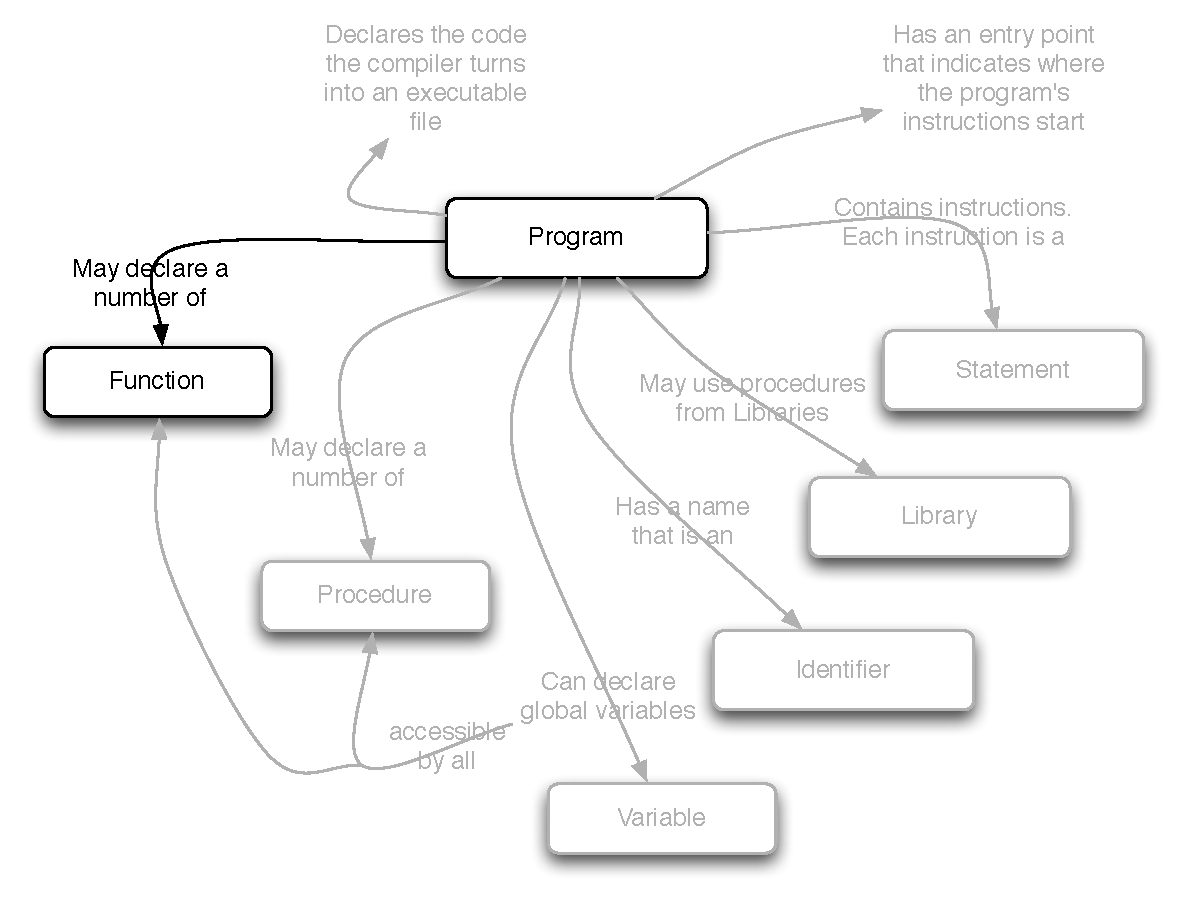
\includegraphics[width=\textwidth]{topics/function-decl/diagrams/ProgramWithFunctions} 
 \caption{Programs can contain Functions}
 \label{fig:function-decl-programs}
\end{figure}


% subsection program_with_functions_ (end)
\clearpage
\subsection{Expression (with Functions)} % (fold)
\label{sub:expression_with_functions_}

\begin{figure}[h]
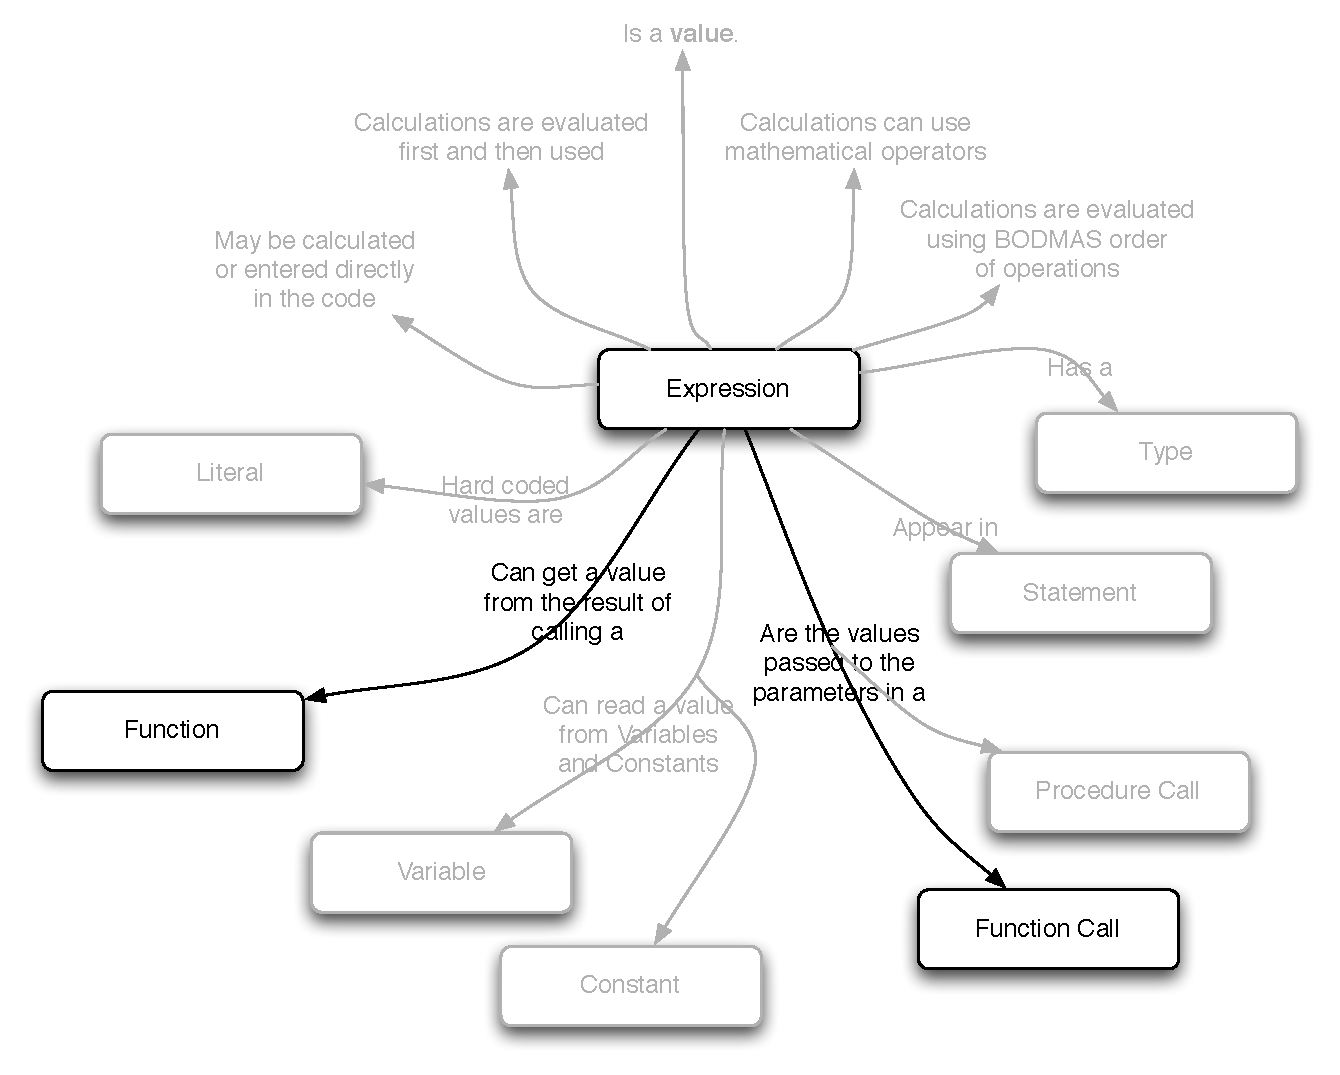
\includegraphics[width=\textwidth]{topics/function-decl/diagrams/Expression} 
 \caption{Expressions can contain values from calling Functions}
 \label{fig:function-decl-expression}
\end{figure}


% subsection expression_with_functions_ (end)

% section function_concepts (end)

% =============
% = C Section =
% =============
\clearpage
\section{Function Declaration in C} % (fold)
\label{sec:function_declaration_in_c}

\clearpage
\subsection{C Function Declaration} % (fold)
\label{sub:c_function_declaration}

\csyntax{csynt:function-decl-function-decl}{a Function}{function-decl/function-decl}

% subsection c_procedure_declaration (end)
\clearpage
\subsection{Return Statement} % (fold)
\label{sub:return_statement}

\csyntax{csynt:function-decl-return-statement}{a Return Statement}{function-decl/return-statement}

% subsection return_statement (end)
\clearpage
\subsection{C Statement (with Return Statement)} % (fold)
\label{sub:c_statement_with_return_statement_}

\csyntax{csynt:function-decl-statement}{Statements (with Return Statement)}{function-decl/statement-with-return}

% subsection c_statement_with_return_statement_ (end)
\clearpage
\subsection{C Function Call} % (fold)
\label{sub:c_function_call}

\csyntax{csynt:function-decl-function-call}{a Function Call}{function-decl/function-call}

% subsection c_procedure_declaration (end)
\clearpage
\subsection{C Procedure Declaration (as Function)} % (fold)
\label{sub:c_procedure_declaration_as_function_}

\csyntax{csynt:function-decl-procedure-decl}{a Procedure (as a Function)}{function-decl/procedure-decl}

% subsection c_procedure_declaration_as_function_ (end)
\clearpage
\subsection{C Program (with Functions)} % (fold)
\label{sub:c_program_with_functions}

\csyntax{csynt:function-decl-program}{a program (with Functions)}{function-decl/program-with-func}

% subsection c_program_with_procedures_ (end)

% section function_declaration_in_c (end)


% chapter function_declaration (end)